
\begin{dsaCharacterSheet}

\renewcommand{\arraystretch}{1}
 \setlength{\tabcolsep}{1pt}

\vspace*{4pt}
\begin{dsaSheetBox}[\textwidth]
    \directlua{common.value_line:render({"AT", "PA", "FK", "INI"}, "18pt")}
\end{dsaSheetBox}

\vspace{-16pt}
\dsaHeading{Waffen \& Kampfwerte}
\vspace{-8pt}

\renewcommand{\arraystretch}{1}
\setlength{\tabcolsep}{1pt}
\normalfont\fontsize{8}{12}\selectfont

\newcommand{\dsaTSHeading}[1]{\normalfont\bfseries\scriptsize #1}

\newcommand{\RS}[1]{%
    \makebox(.7cm,.8em)[c]{\dsaHeroVal{ruestung.#1}\hspace{-2.5pt}}
}

\begin{dsaSheetBox}[\textwidth]
    \begin{NiceTabular}{p{4.8cm}|x{1.8cm}@{/}x{0.5cm}|x{1cm}|x{1.4cm}|x{0.8cm}@{/}x{0.7cm}|x{1cm}|x{0.6cm}@{/}x{0.6cm}|x{0.8cm}|x{0.8cm}|x{1.4cm}|x{0.5cm}|x{0.5cm}}
    \CodeBefore\rowcolors{2}{white}{gray!30}\Body
        \dsaTHeading{Nahkampfwaffe} &
        \multicolumn{2}{c|}{\dsaTHeading{Typ/eBE}} &
        \dsaTHeading{DK} &
        \dsaTHeading{TP} &
        \multicolumn{2}{c|}{\dsaTHeading{TP/KK}} &
        \dsaTHeading{INI} &
        \multicolumn{2}{c|}{\dsaTHeading{WM}} &
        \dsaTHeading{AT} &
        \dsaTHeading{PA} &
        \dsaTHeading{TP} &
        \multicolumn{2}{c}{\dsaTHeading{BF}} \\ \Xhline{2\arrayrulewidth}
        \directlua{
            common.inner_rows(data.nahkampf, 15)
        } \\ \Xhline{3\arrayrulewidth}
    \end{NiceTabular}

    \vspace{2pt}
    \begin{tabular}{p{\textwidth-1.33\tabcolsep}}
        \directlua{
            common.labelled_rows(data.sf.nahkampf, "Sonderfertigkeiten")
        }
    \end{tabular}
\end{dsaSheetBox}

\begin{dsaSheetBox}[\textwidth]
    \begin{NiceTabular}{p{4.5cm}|x{1.4cm}@{/}x{0.5cm}|x{1.4cm}|x{0.6cm}@{/}x{0.6cm}@{/}x{0.6cm}@{/}x{0.6cm}@{/}x{0.6cm}|x{0.6cm}@{/}x{0.6cm}@{/}x{0.6cm}@{/}x{0.6cm}@{/}x{0.6cm}|x{0.8cm}|x{0.5cm}|x{0.5cm}|x{0.5cm}|x{0.5cm}}
    \CodeBefore\rowcolors{2}{white}{gray!30}\Body
        \dsaTHeading{Fernkampfwaffe} &
        \multicolumn{2}{c|}{\dsaTHeading{Typ/eBE}} &
        \dsaTHeading{TP} &
        \multicolumn{5}{c|}{\dsaTHeading{Entfernungen}} &
        \multicolumn{5}{c|}{\dsaTHeading{TP/Entfernung}} &
        \dsaTHeading{FK} &
        \multicolumn{4}{c}{\dsaTHeading{Geschosse}} \\ \Xhline{2\arrayrulewidth}
        \directlua{
            common.inner_rows(data.fernkampf, 19)
        } \\ \Xhline{3\arrayrulewidth}
    \end{NiceTabular}

    \vspace{2pt}
    \begin{tabular}{p{\textwidth-1.33\tabcolsep}}
        \directlua{
            common.labelled_rows(data.sf.fernkampf, "Sonderfertigkeiten")
        }
    \end{tabular}
\end{dsaSheetBox}

\begin{minipage}{12.6cm}
	\begin{dsaSheetBox}[\textwidth]
        \begin{NiceTabular}{p{4.85cm}|x{0.6cm}@{/}x{0.6cm}|x{1cm}|x{1cm}|x{1cm}|x{2.5cm}}
        \CodeBefore\rowcolors{2}{white}{gray!30}\Body
            \dsaTHeading{Waffenloser Kampf} &
            \multicolumn{2}{c|}{\dsaTHeading{TP/KK}} &
            \dsaTHeading{INI} &
            \dsaTHeading{AT} &
            \dsaTHeading{PA} &
            \dsaTHeading{TP(A)} \\ \Xhline{2\arrayrulewidth}
            \directlua{
                kampfbogen.waffenlos(data.waffenlos)
            } \\ \Xhline{3\arrayrulewidth}
        \end{NiceTabular}

        \vspace{2pt}
        \begin{tabular}{p{\textwidth-1.33\tabcolsep}}
            \directlua{
                common.labelled_rows(data.sf.waffenlos, "Sonderfertigkeiten")
            }
        \end{tabular}
    \end{dsaSheetBox}
	\vspace{-28pt}
    \begin{center}
        \LARGE\bfseries\textmansontt{\shadowtext{Schild / Parierwaffe}}%
    \end{center}%
    \vspace{-4pt}

    \begin{dsaSheetBox}
        \begin{NiceTabular}{p{4.85cm}|x{2.6cm}|x{1cm}|x{0.6cm}@{/}x{0.6cm}|x{0.8cm}|x{0.5cm}|x{0.5cm}}
        \CodeBefore\rowcolors{2}{white}{gray!30}\Body
            \dsaTHeading{Name} &
            \dsaTHeading{Typ} &
            \dsaTHeading{INI} &
            \multicolumn{2}{c|}{\dsaTHeading{WM}} &
            \dsaTHeading{PA} &
            \multicolumn{2}{c}{\dsaTHeading{BF}} \\ \Xhline{2\arrayrulewidth}
            \directlua{
                common.inner_rows(data.schilde, 8)
            } \\ \Xhline{3\arrayrulewidth}%
        \end{NiceTabular}

        \vspace{2pt}
        \footnotesize\normalfont\bfseries\centering
        \directlua{
            common.checkboxlist({
                {"Linkhand (PA+1)", data.schilde.linkhand},
                {{"Schildkampf I (PA+2)", "II (PA+2)"}, data.schilde.schildkampf},
                {{"Parierwaffen I", "II"}, data.schilde.parierwaffen}
            })
        }
    \end{dsaSheetBox}

	\vspace{4pt}
	\begin{minipage}{6cm}
		\begin{center}
            \LARGE\bfseries\textmansontt{\shadowtext{Rüstung}}%
        \end{center}%
        \vspace{-4pt}

        \begin{dsaSheetBox}
            \begin{NiceTabular}{p{3.8cm}|x{0.8cm}|x{0.8cm}}
            \CodeBefore\rowcolors{2}{white}{gray!30}\Body
                \dsaTHeading{Rüstungsstück} &
                \dsaTHeading{RS} &
                \dsaTHeading{BE} \\ \Xhline{2\arrayrulewidth}
                \directlua{
                    common.inner_rows(data.ruestung, 3)
                } \\ \Xhline{2\arrayrulewidth}
                \normalfont\bfseries\scriptsize Summe &
                \directlua{tex.sprint(data:cur("RS"))} & \directlua{tex.sprint(data:cur("BE"))} \\ \Xhline{2\arrayrulewidth}
                \multicolumn{2}{l|}{
                    \normalfont\scriptsize\bfseries Rüstungsgewöhnung
                    \directlua{
                        common.checkboxlist({
                            {{"I", "II", "III"}, data.ruestung.gewoehnung}
                        })
                    }

                } & \directlua{tex.sprint(-2, data.ruestung.be)}
            \end{NiceTabular}
        \end{dsaSheetBox}
	\end{minipage}
	\begin{minipage}{6.5cm}
		\begin{center}
            \LARGE\bfseries\textmansontt{\shadowtext{Ausweichen}}%
        \end{center}%
        \vspace{-3.5pt}

        \begin{dsaSheetBox}
            \setlength{\tabcolsep}{0pt}
            \tiny\normalfont\bfseries
            \begin{tabular}{x{1cm}p{0.3cm}x{0.7cm}p{0.3cm}x{2.5cm}p{0.3cm}x{1cm}}
                \multicolumn{2}{l}{\scriptsize PA-Basis} & \scriptsize BE & & \scriptsize SF Ausweichen & & \scriptsize Summe \\
                \normalsize \directlua{tex.sprint(-2, data:cur("PA"))} &
                \normalsize $-$ &
                \normalsize \directlua{tex.sprint(-2, data.ruestung.be)} &
                \normalsize $+$ &
                \begin{minipage}{2.5cm}
                    \centering
                    \directlua{common.checkboxlist({{{"I", "II", "III"}, data.ausweichen.sf}})} \\
                    jeweils +3 \\
                    Flink (+1) / Behäbig (-1)?
                \end{minipage}
                & \normalsize $=$ &
                \normalsize \directlua{tex.sprint(-2, data.ausweichen[1])}
                \\ \Xcline{1-1}{3\arrayrulewidth} \Xcline{3-3}{3\arrayrulewidth} \Xcline{7-7}{3\arrayrulewidth}
                 & & & \multicolumn{3}{c}{Akrobatik (+$\lfloor(\mathrm{TaW}-9) / 3 \rfloor $)?} &
            \end{tabular}
        \end{dsaSheetBox}

		\vspace{-4.8pt}
		\begin{center}
            \LARGE\bfseries\textmansontt{\shadowtext{Wunden}}%
        \end{center}%
        \vspace{-3pt}

        \begin{dsaSheetBox}
            \centering
            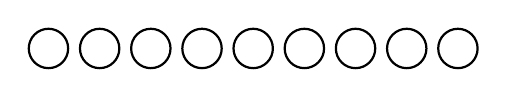
\begin{tikzpicture}
                \filldraw[fill=white, draw=black, thick] (1,1) circle (0.25cm);
                \filldraw[fill=white, draw=black, thick] (1.65,1) circle (0.25cm);
                \filldraw[fill=white, draw=black, thick] (2.3,1) circle (0.25cm);
                \filldraw[fill=white, draw=black, thick] (2.95,1) circle (0.25cm);
                \filldraw[fill=white, draw=black, thick] (3.6,1) circle (0.25cm);
                \filldraw[fill=white, draw=black, thick] (4.25,1) circle (0.25cm);
                \filldraw[fill=white, draw=black, thick] (4.9,1) circle (0.25cm);
                \filldraw[fill=white, draw=black, thick] (5.55,1) circle (0.25cm);
                \filldraw[fill=white, draw=black, thick] (6.2,1) circle (0.25cm);
            \end{tikzpicture} \\
            \scriptsize\normalfont\bfseries je Wunde AT, PA, FK, GE, INI - 2, GS - 1
        \end{dsaSheetBox}
	\end{minipage}
\end{minipage}
\begin{minipage}{\textwidth-12.6cm-\fboxsep}
    \normalfont\bfseries
    \begin{tikzpicture}
        \begin{scope}[on background layer]
            \node[anchor=south west,inner sep=0] at (0,0) {
\includegraphics[width=6cm]{../img/silhouette.png}};
        \end{scope}

        \node(kopf) at (3.4, 10) {\RS{kopf}};
        \begin{scope}[on background layer]
            \path[fill=white, draw=black] ([yshift=0.1cm, xshift=0.2cm]kopf.north west) -- ([xshift=0.2cm]kopf.west) to[out=270, in=155] ([yshift=-0.1cm]kopf.south) to[out=25, in=270] ([xshift=-0.2cm]kopf.east) -- ([yshift=0.1cm, xshift=-0.2cm]kopf.north east) -- cycle;
        \end{scope}
        \node[below=2pt of kopf] {Ko};

        \filldraw[fill=white, draw=black] ([yshift=0.4cm]kopf.north) circle (0.2cm);
        \filldraw[fill=white, draw=black] ([yshift=0.4cm, xshift=0.5cm]kopf.north) circle (0.2cm);
        \filldraw[fill=white, draw=black] ([yshift=0.4cm, xshift=-0.5cm]kopf.north) circle (0.2cm);

        \node[minimum width=.4cm](brust) at (2.7, 8) {\RS{brust}};
        \begin{scope}[on background layer]
            \path[fill=white, draw=black] ([yshift=0.1cm, xshift=0.2cm]brust.north west) -- ([xshift=0.2cm]brust.west) to[out=270, in=155] ([yshift=-0.1cm]brust.south) to[out=25, in=270] ([xshift=-0.2cm]brust.east) -- ([yshift=0.1cm, xshift=-0.2cm]brust.north east) -- cycle;
        \end{scope}
        \node[below=2pt of brust] {Br};
        \node[right=-4pt of brust](rucken) {\RS{ruecken}};
        \begin{scope}[on background layer]
            \path[fill=white, draw=black] ([yshift=0.1cm, xshift=0.2cm]rucken.north west) -- ([xshift=0.2cm]rucken.west) to[out=270, in=155] ([yshift=-0.1cm]rucken.south) to[out=25, in=270] ([xshift=-0.2cm]rucken.east) -- ([yshift=0.1cm, xshift=-0.2cm]rucken.north east) -- cycle;
        \end{scope}
        \node[below=2pt of rucken] {Rü};

        \filldraw[fill=white, draw=black] ([yshift=0.4cm]$(brust.north)!0.5!(rucken.north)$) circle (0.2cm);
        \filldraw[fill=white, draw=black] ([yshift=0.4cm, xshift=0.5cm]$(brust.north)!0.5!(rucken.north)$) circle (0.2cm);
        \filldraw[fill=white, draw=black] ([yshift=0.4cm, xshift=-0.5cm]$(brust.north)!0.5!(rucken.north)$) circle (0.2cm);

        \node(larm) at (5.6, 6.4) {\RS{linker_arm}};
        \begin{scope}[on background layer]
            \path[fill=white, draw=black] ([yshift=0.1cm, xshift=0.2cm]larm.north west) -- ([xshift=0.2cm]larm.west) to[out=270, in=155] ([yshift=-0.1cm]larm.south) to[out=25, in=270] ([xshift=-0.2cm]larm.east) -- ([yshift=0.1cm, xshift=-0.2cm]larm.north east) -- cycle;
        \end{scope}
        \node[below=2pt of larm] {LA};

        \filldraw[fill=white, draw=black] ([yshift=0.5cm, xshift=0.1cm]larm.north west) circle (0.2cm);
        \filldraw[fill=white, draw=black] ([yshift=1cm, xshift=-0.15cm]larm.north west) circle (0.2cm);
        \filldraw[fill=white, draw=black] ([yshift=1.5cm, xshift=-0.4cm]larm.north west) circle (0.2cm);

        \node(rarm) at (0.5, 6.7) {\RS{rechter_arm}};
        \begin{scope}[on background layer]
            \path[fill=white, draw=black] ([yshift=0.1cm, xshift=0.2cm]rarm.north west) -- ([xshift=0.2cm]rarm.west) to[out=270, in=155] ([yshift=-0.1cm]rarm.south) to[out=25, in=270] ([xshift=-0.2cm]rarm.east) -- ([yshift=0.1cm, xshift=-0.2cm]rarm.north east) -- cycle;
        \end{scope}
        \node[below=2pt of rarm] {RA};

        \filldraw[fill=white, draw=black] ([yshift=0.2cm, xshift=0.1cm]rarm.north east) circle (0.2cm);
        \filldraw[fill=white, draw=black] ([yshift=0.6cm, xshift=0.5cm]rarm.north east) circle (0.2cm);
        \filldraw[fill=white, draw=black] ([yshift=1cm, xshift=0.9cm]rarm.north east) circle (0.2cm);

        \node(bauch) at (3, 6) {\RS{bauch}};
        \begin{scope}[on background layer]
            \path[fill=white, draw=black] ([yshift=0.1cm, xshift=0.2cm]bauch.north west) -- ([xshift=0.2cm]bauch.west) to[out=270, in=155] ([yshift=-0.1cm]bauch.south) to[out=25, in=270] ([xshift=-0.2cm]bauch.east) -- ([yshift=0.1cm, xshift=-0.2cm]bauch.north east) -- cycle;
        \end{scope}
        \node[below=2pt of bauch] {Ba};

        \filldraw[fill=white, draw=black] ([yshift=0.4cm]bauch.north) circle (0.2cm);
        \filldraw[fill=white, draw=black] ([yshift=0.4cm, xshift=0.5cm]bauch.north) circle (0.2cm);
        \filldraw[fill=white, draw=black] ([yshift=0.4cm, xshift=-0.5cm]bauch.north) circle (0.2cm);

        \node(rbein) at (1.9, 1.5) {\RS{rechtes_bein}};
        \begin{scope}[on background layer]
            \path[fill=white, draw=black] ([yshift=0.1cm, xshift=0.2cm]rbein.north west) -- ([xshift=0.2cm]rbein.west) to[out=270, in=155] ([yshift=-0.1cm]rbein.south) to[out=25, in=270] ([xshift=-0.2cm]rbein.east) -- ([yshift=0.1cm, xshift=-0.2cm]rbein.north east) -- cycle;
        \end{scope}
        \node[below=2pt of rbein] {RB};

        \filldraw[fill=white, draw=black] ([yshift=0.8cm, xshift=0.2cm]rbein.north) circle (0.2cm);
        \filldraw[fill=white, draw=black] ([yshift=1.6cm, xshift=0.3cm]rbein.north) circle (0.2cm);
        \filldraw[fill=white, draw=black] ([yshift=2.4cm, xshift=0.4cm]rbein.north) circle (0.2cm);

        \node(lbein) at (5.1, 1.3) {\RS{linkes_bein}};
        \begin{scope}[on background layer]
            \path[fill=white, draw=black] ([yshift=0.1cm, xshift=0.2cm]lbein.north west) -- ([xshift=0.2cm]lbein.west) to[out=270, in=155] ([yshift=-0.1cm]lbein.south) to[out=25, in=270] ([xshift=-0.2cm]lbein.east) -- ([yshift=0.1cm, xshift=-0.2cm]lbein.north east) -- cycle;
        \end{scope}
        \node[below=2pt of lbein] {LB};

        \filldraw[fill=white, draw=black] ([yshift=0.8cm, xshift=-0.3cm]lbein.north) circle (0.2cm);
        \filldraw[fill=white, draw=black] ([yshift=1.6cm, xshift=-0.6cm]lbein.north) circle (0.2cm);
        \filldraw[fill=white, draw=black] ([yshift=2.4cm, xshift=-0.9cm]lbein.north) circle (0.2cm);
    \end{tikzpicture}
\end{minipage}

\vspace{-10pt}
\begin{center}%
    \LARGE\bfseries\textmansontt{\shadowtext{Lebensenergie, Ausdauer, etc.}}%
\end{center}%
\vspace{-12pt}

\begin{dsaSheetBox}
    \begin{NiceTabular}{p{3cm}|x{1cm}|x{1cm}|x{1cm}|x{1cm}|p{11.1cm}}
    \CodeBefore\rowcolors{2}{white}{gray!30}\Body
        & \dsaTSHeading{max.} & \dsaTSHeading{1/2} & \dsaTSHeading{1/3} & \dsaTSHeading{1/4} & \normalfont\bfseries\scriptsize\hspace{2pt} aktuell \\ \Xhline{2\arrayrulewidth}
        \directlua{kampfbogen.energieleiste("Lebensenergie", data:cur("LE"))} \\ \hline
        \directlua{kampfbogen.energieleiste("Ausdauer", data:cur("AU"))}
        \directlua{kampfbogen.optionalleiste("Astralenergie", data:cur("AE"))}
        \directlua{kampfbogen.optionalleiste("Karmaenergie", data:cur("KE"))}
    \end{NiceTabular}
\end{dsaSheetBox}

\end{dsaCharacterSheet}